\subsection[Plastic plate - Drucker-Prager plasticity (2D)]{Plastic plate - Drucker-Prager plasticity, enhanced strain element (2D)}

\subsubsection*{Problem definition}

In this application, we analyze a plane strain biaxial failure
de\-for\-ma\-tion problem with triangle and quadrilateral
elements, correspondingly. We use an enhanced strain approximation
to simulate the displacement discontinuity after failure appears.
Neighbor relationships of an element object are essential data for
constructing the deforming mesh and to determinate the propagation
orientation of the discontinuity in the failure analysis.

From the view point of bifurcation theory, strain localization is a
bifurcation phenomenon, which takes place when the velocity field
moves away from the branch of continuous solutions and takes a new
path of discontinuous solutions. If standard finite element is
applied to this problem, we have to refine mesh adaptively near the
localization area. Otherwise, the system equation is ill-posed. The
strong discontinuity approach with enhanced strain element avoids
the ill-posed system equations and therefore avoid mesh sensitive of
the analysis \cite{SanWri84}.

The set-up of the biaxial compression problem as proposed by
\cite{Bo00} is shown in Fig. \ref{fig:biaxial}. The geometry of the
specimen is simplified to a rectangle with size of 1m$\times$3m.
\begin{figure}[!htb]
\center
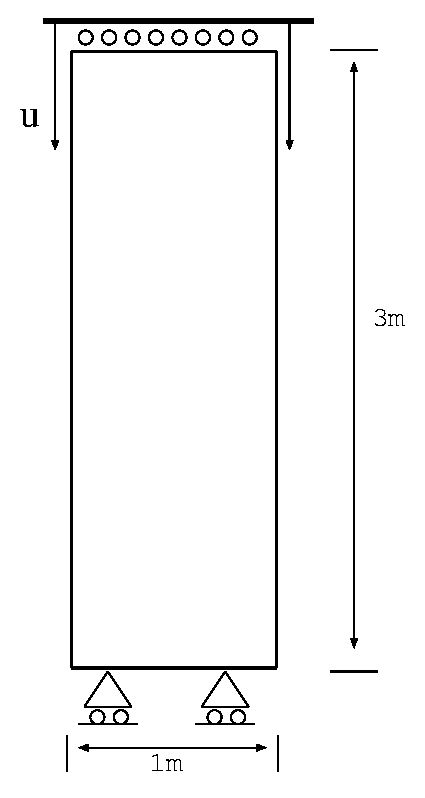
\includegraphics[scale=0.45]{M/biaxial.eps}
\caption{Plane strain biaxial test}
 \label{fig:biaxial}
\end{figure}

\subsubsection*{Boundary conditions}

The bottom of the specimen is placed on horizontal roll supporters.
While the top of it is only allowed to a vertical down movement
$u_z$. Both lateral sides are considered to be traction free.

\subsubsection*{Material properties}

The non-associative flow rule is adopted for the Drucker-Prager model. All material parameters are given in Table (\ref{ex1:tableDP})

\begin{table}[H]
\centering
\begin{tabular}{lll}
\hline \hline
Parameter   &  Unit  & Value\\
\hline
  Young's modulus &  $kPa$ &  $2\times10^4$ \\
\hline\hline
  Poisson ratio & - &  0.4 \\
\hline
  Parameter $\alpha$  & - & 0.233345 (30$^\circ$ friction angle)\\
\hline
  Parameter $\beta$  & - &  0.141421 (16.53$^\circ$ dilatancy angle)\\
\hline
  Initial stress $\sigma_0$ & $kPa$ &  29.69 (20 of initial cohesion)\\
\hline
  Hardening modulus $H$ & $kPa$ &  100\\
\hline
  Localized softening modulus $H_{\delta}$ & $kPa$ & -1000, varying\\
\hline \hline
\end{tabular}
\caption{Material parameters of the plane strain biaxial test}
\label{ex1:tableDP}
\end{table}

\subsubsection*{Results}
Fig. \ref{fig:loc} shows the deformed sample exhibiting localization. Fig. \ref{fig:vreact} depicts the stress
reaction at the top surface due to the displacement load. The results agrees with what given in \cite{Bo00}

\begin{figure}[H]
\begin{center}
\includegraphics[scale=0.35]{M/m_sdc.eps}
\end{center}
\caption{Vertical reaction of the top}.
 \label{fig:loc}
\end{figure}
\begin{figure}[H]
\begin{center}
\includegraphics[scale=0.35]{M/m_sdc_s_u.eps}
\end{center}
\caption{Vertical reaction of the top}.
 \label{fig:vreact}
\end{figure}

\subsubsection*{Benchmark deposit}
\begin{tabular}{|l|l|l|}
  \hline
  Benchmark & Problem type & Path in benchmark deposit \\
  \hline
 \emph{m\_sdc} & M & benchmarks\verb \M\ \\
  \hline
\end{tabular}

